\documentclass[10pt]{article}
\usepackage[polish]{babel}
\usepackage[utf8]{inputenc}
\usepackage[T1]{fontenc}
\usepackage{graphicx}
\usepackage[export]{adjustbox}
\graphicspath{ {./images/} }

\title{LIGA MATEMATYCZNA im. Zdzisława Matuskiego PAŹDZIERNIK 2019 SZKOŁA PODSTAWOWA \\
 klasy IV - VI }

\author{}
\date{}


\begin{document}
\maketitle
\section*{ZADANIE 1.}
W pola diagramu wpisano siedem kolejnych liczb naturalnych (w kolejności od najmniejszej do największej). Suma trzech pierwszych liczb jest równa 69. Ile liczb podzielnych przez 3 znajduje się wśród tych liczb?\\
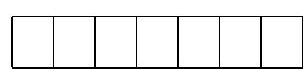
\includegraphics[max width=\textwidth, center]{2024_11_21_a97cad5a8f63b3478346g-1}

\section*{ZADANIE 2.}
W regatach żeglarskich wzięło udział 48 chłopców. Sześciu z nich przybyło z jednym bratem, dziewięciu z dwoma braćmi i czterech z trzema braćmi. Pozostali chłopcy przybyli bez rodzeństwa. Z ilu rodzin było tych 48 chłopców?

\section*{ZADANIE 3.}
Prostokątną kartkę papieru podzielono na kwadraty i prostokąt A. Długość boku kwadratu B jest równa 4. Oblicz obwód prostokąta A.\\
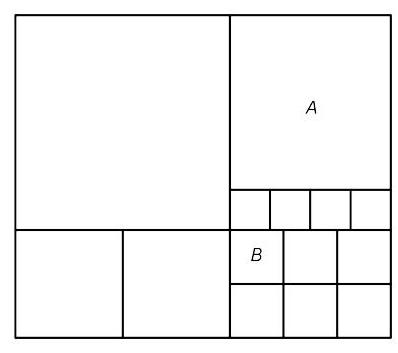
\includegraphics[max width=\textwidth, center]{2024_11_21_a97cad5a8f63b3478346g-1(1)}

\section*{ZADANIE 4.}
Dziewczynki zbierały koniczynę na łące. Niektóre gałązki miały po trzy listki, a inne po cztery. Razem zebrały 39 gałązek, na których było łącznie 128 listków. Ile gałązek czterolistnej koniczyny zebrały dziewczynki?

\section*{ZADANIE 5.}
Ile jest liczb czterocyfrowych o sumie cyfr równej 3? Czy suma tych liczb jest liczbą podzielną przez 9? A przez 3?


\end{document}